\documentclass[a4paper,12pt]{article}
\usepackage{amsmath} % For equations
\usepackage{amssymb} % For mathematical symbols
\usepackage{graphicx} % For figures (optional)
\usepackage{natbib} % For references
\usepackage[left=1in, right=1in, top=1in, bottom=1in]{geometry} % Margins

\title{Statistical Arbitrage in the Vietnamese Stock Market: Long-only Stock Approach}
\author{Hieu Cao}
\date{\today}

\begin{document}

\maketitle

\section*{Abstract}
Financial markets are inherently noisy, providing opportunities for algorithmic strategies to exploit pricing inefficiencies. This report develops a statistical arbitrage strategy inspired by Avellaneda and Lee, adapted for the Vietnamese stock market, where short selling of individual stocks is prohibited. I propose longing a basket of stocks and shorting the VN30F1M futures contract to capture mean-reverting relationships. I formed combinations by employing clustering techniques, the Johansen cointegration test, and generate signals by using the s-score of the Ornstein-Uhlenbeck process. After the backtesting, I found that the key things depends on how the trading signal is designed and additional efforts (time and computational power) should be implemented for the best performance of the model.

\section{Introduction}
\subsection{Hypothesis} 
In the Vietnamese stock market, dominated by retail investors, stocks exhibit exaggerated price movements due to overreactions to news or sentiment. These deviations from fundamental values result in wider spreads between stock baskets and the VN30F1M futures, which revert to their historical mean, enabling profitable trades via algorithmic mean-reversion strategies. 

\subsection{Key Idea}
Statistical arbitrage is a prevalent strategy in modern algorithmic trading, offering market-neutral returns that are independent of overall market movements. Investors are drawn to this alternative investment approach due to its diversification benefits and the potential for high rewards with relatively low risk, akin to earning high interest from a bank deposit but with greater upside potential.

Statistical arbitrage leverages statistical techniques to profit from pricing inefficiencies in financial markets, typically through mean-reverting portfolios. A well-known method, pairs trading, involves trading two correlated securities—longing one and shorting the other—when their price relationship deviates, expecting convergence. This is modeled as:
\[
\frac{dP_t}{P_t} = \alpha \, dt + \beta \frac{dQ_t}{Q_t} + dX_t,
\]
where \( P_t \) and \( Q_t \) are the prices of two stocks, \( \alpha \) is a drift term (often negligible), \( \beta \) is the hedge ratio, and \( X_t \) is a mean-reverting residual driving trading decisions.

In Vietnam, however, regulatory restrictions prohibit short selling of individual stocks, rendering classical pairs trading impractical. To address this, the proposed strategy involves longing a basket of stocks and shorting the VN30F1M futures contract, thereby maintaining the market-neutral principle. The objective is to identify combinations of the form:
\[
\text{VN30F1M} = \text{intercept} + \sum_{i} \beta_i \cdot \text{stock}_i + \text{residual},
\]
where the residual is stationary. This approach enhances profitability in a constrained market, a critical consideration for investors seeking diversified, low-risk strategies.

The combination formation process begins with clustering stocks based on a 60-day window of residuals, derived from an ordinary least squares (OLS) regression of each stock against the VN30F1M futures. Stocks are grouped into smaller clusters to improve computational efficiency. Subsequently, the Johansen cointegration test is applied to build tradable combinations, which are then validated and checked for similarity to avoid redundancy. Finally, the residuals are modeled using the Ornstein-Uhlenbeck (O-U) process to compute the s-score, which forms the basis for generating trading signals.

\section{Related Work}
Statistical arbitrage has a well-established foundation in financial literature. Avellaneda and Lee (2010) formalized pairs trading using cointegration and the Ornstein-Uhlenbeck (O-U) process, modeling the spread \( X_t \) as:
\[
dX_t = \kappa (\mu - X_t) \, dt + \sigma \, dW_t,
\]
where \( \kappa \) is the mean reversion speed, \( \mu \) is the long-term mean, and \( \sigma \) is the volatility, with trading signals derived from the s-score. To estimate the O-U parameters, the process \( X_t \) can be approximated using an AR(1) model by solving the 1-lag regression:
\[
X_{n+1} = a + b X_n + \theta_{n+1},
\]


A group of students from Standford (Lu, Parulekar, Xu, 2018) introduced the idea of clustering and the Johansen Test for the cointegration instead of the traditional Engel Granger cointegration test because Johansens test allows more than one cointegration relationship, for measuring cointegration between many stocks and the future. 

The Johensen test is a key differentiator in the proposed strategy, as opposed to methods like principal component analysis (PCA) or linear regression used in other approaches. Additionally, the Johansen test facilitates the determination of appropriate weights for the stock combinations, whereas Lu, Parulekar, and Xu relied on the mean reversion speed \( \kappa \) for similar purposes.

\section{Forming Combinations}
Our strategy is implemented via two core components: data handling and combination formation, detailed below.

\subsection{Data Handling}
The \texttt{DataHandler} class manages price data and clusters stocks based on their residuals relative to the futures.
\begin{itemize}
    \item \textbf{Data}: from Algotrade Database ( 01/06/2021-31/12/2024) 
    \item \textbf{Residual Computation}: For each stock \( S_t \), an OLS regression against the futures \( F_t \) over a 60-day window yields:
    \[
    S_t = \alpha + \beta F_t + \epsilon_t,
    \]
    where \( \epsilon_t \) is the residual series stored for clustering.
    \item \textbf{Clustering}: KMeans groups stocks by residual similarity, with the number of clusters (up to 10) optimized via the silhouette score. Clusters update every 3 days or upon significant futures price shifts.
\end{itemize}


\subsection{Steps to Form a Combination}
The formation of a cointegrated combination involves several methodical steps, as implemented in the \texttt{Combination\_Formations} class. Below, I describe each step, integrating detailed explanations of the Johansen test where it is utilized.

\subsubsection{Step 1: Pairwise Candidate Selection}
The process begins by identifying stocks that are individually cointegrated with the futures contract, using pairwise Johansen tests. This is implemented in the \texttt{get\_pairwise\_candidates} method.

\begin{itemize}
    \item \textbf{Procedure}: For each stock in a given pool (e.g., a cluster of stocks), historical price data for the futures and the stock over an estimation window is extracted. The Johansen cointegration test is performed on this pair using the \texttt{coint\_johansen} function from the \texttt{statsmodels} library, with a deterministic trend (\texttt{det\_order=1}) and one lag difference (\texttt{k\_ar\_diff=1}).
    \item \textbf{Criterion}: If the trace statistic from the test exceeds the critical value at the specified confidence level (e.g., 90\% or 95\%, indexed by \texttt{confidence\_level}), the stock is deemed a candidate. Candidates are then sorted by their trace statistics in descending order, prioritizing stocks with stronger evidence of cointegration.
\end{itemize}

\textbf{Johansen Test}:

The Johansen test assesses cointegration among multiple time series, determining if they share a long-run equilibrium relationship despite being individually non-stationary. Here, it is applied to a pair: the futures price and a single stock price.

- \textbf{Concept}: Cointegration implies that a linear combination of non-stationary series is stationary, indicating a stable relationship. For two series, there can be at most one cointegrating relationship.
- \textbf{Mathematical Formulation}: The test is based on the Vector Error Correction Model (VECM):
  \[
  \Delta \mathbf{y}_t = \Pi \mathbf{y}_{t-1} + \sum_{i=1}^{p-1} \Gamma_i \Delta \mathbf{y}_{t-i} + \mathbf{\epsilon}_t
  \]
  where \(\mathbf{y}_t = (y_{1t}, y_{2t})'\) (futures and stock prices), \(\Delta \mathbf{y}_t = \mathbf{y}_t - \mathbf{y}_{t-1}\), \(\Pi = \alpha \beta'\) is the long-run coefficient matrix, \(\Gamma_i\) are short-run adjustment matrices, and \(\mathbf{\epsilon}_t \sim N(0, \Sigma)\). The rank of \(\Pi\) (denoted \(r\)) indicates the number of cointegrating relationships: \(r = 0\) (no cointegration), \(r = 1\) (one cointegrating relationship).

- \textbf{Trace Statistic}: The trace test evaluates the null hypothesis \(H_0: r \leq r_0\) against \(H_1: r > r_0\). The statistic is:
  \[
  \lambda_{\text{trace}}(r_0) = -T \sum_{i=r_0+1}^{k} \ln(1 - \hat{\lambda}_i)
  \]
  where \(T\) is the number of observations, \(k = 2\) (number of series), and \(\hat{\lambda}_i\) are eigenvalues from the \(\Pi\) matrix, ordered \(\hat{\lambda}_1 > \hat{\lambda}_2\). For \(r_0 = 0\), if \(\lambda_{\text{trace}}(0) > \text{critical value}\), we reject \(H_0\), indicating at least one cointegrating relationship.

- \textbf{Eigenvalues}: The eigenvalues \(\hat{\lambda}_i\) are derived by solving the eigenvalue problem of the matrix formed from the residuals of regressions of \(\Delta \mathbf{y}_t\) and \(\mathbf{y}_{t-1}\) on lagged differences. They measure the strength of cointegration, with larger values indicating stronger relationships.

In the code, \texttt{result.lr1[0]} is the trace statistic for \(r = 0\), compared against \texttt{result.cvt[0, confidence\_level]}, the critical value.

\subsubsection{Step 2: Greedy Combination Building}
Next, a combination is constructed greedily from the candidate stocks, as implemented in the \texttt{build\_combination\_greedy} method.

\begin{itemize}
    \item \textbf{Procedure}: Start with the top candidate stock (highest trace statistic from Step 1). Iteratively add the next candidate, testing the entire set (futures plus selected stocks) with the Johansen test. A stock is included if:
    \begin{enumerate}
        \item The trace statistic exceeds the critical value at the confidence level.
        \item The improvement in the trace statistic, defined as \(\frac{\text{new trace} - \text{current trace}}{\text{current trace}}\), exceeds the \texttt{improvement\_threshold} (default 0.03).
        \item All betas (weights derived from the eigenvector) are positive.
    \end{enumerate}
    This continues until no more stocks improve the combination or the maximum number of stocks (\texttt{max\_stocks}, default 10) is reached. To enhance robustness, the process tries multiple starting points (top 5 candidates by default) and selects the combination with the highest trace statistic.
\end{itemize}

\textbf{Johansen Test Explanation}:

Here, the Johansen test is applied to a multivariate set: the futures and multiple stocks.

- \textbf{Concept}: Unlike the pairwise case, multiple series can have up to \(k-1\) cointegrating relationships, where \(k\) is the number of series. The goal is to find a combination where the futures is cointegrated with a portfolio of stocks.

- \textbf{Mathematical Formulation}: For \(\mathbf{y}_t = (y_{0t}, y_{1t}, \ldots, y_{mt})'\) (futures and \(m\) stocks), the VECM is as above. The rank \(r\) of \(\Pi\) ranges from 0 to \(m\). We seek \(r \geq 1\), ensuring at least one cointegrating vector.


- \textbf{Eigenvalues and Eigenvectors}: Eigenvalues \(\hat{\lambda}_i\) are computed as in Step 1, but for a larger system. The eigenvector \(\mathbf{v} = (v_0, v_1, \ldots, v_m)'\) corresponding to the largest eigenvalue (\texttt{result.evec[:, 0]}) defines the cointegrating vector. Betas are calculated as \(\beta_i = -\frac{v_i}{v_0}\) for \(i = 1, \ldots, m\), normalizing the futures’ coefficient to 1.

\subsubsection{Step 3: Validation}
The constructed combination is validated in the \texttt{validate\_combination} method to ensure its robustness.

\begin{itemize}
    \item \textbf{Procedure}: Perform the Johansen test on the full set (futures and selected stocks) with a stricter confidence level (\texttt{confidence\_level\_joh\_final}, typically one level higher than initial tests, e.g., 95\% instead of 90\%). Additional checks include:
    \begin{enumerate}
        \item All betas (\(\beta_i = -\frac{v_i}{v_0}\)) are positive.
        \item The residuals (futures price minus synthetic portfolio) are stationary, verified by the Augmented Dickey-Fuller (ADF) test with a p-value below \texttt{adf\_significance} (default 0.05).
        \item The 95th percentile of absolute residuals does not exceed \texttt{residual\_threshold} (default 0.3) times the average futures price.
    \end{enumerate}
    If all conditions are met, the combination is parameterized with an intercept and betas.
\end{itemize}


\subsubsection{Step 4: Similarity Check and Finalization}
Before adding the combination to the active list, the \texttt{add\_combination\_if\_not\_similar} method checks its residuals against existing combinations using Pearson correlation. If the correlation exceeds \texttt{correlation\_threshold} (default 0.6), and the existing combination is mature (beyond \texttt{min\_trading\_days}), it may be replaced if the new combination’s residuals are more stationary.
\section{Signal Generation}
\subsection{Ornstein-Uhlenbeck Process Fitting}
The signal generation begins by fitting an OU process to the residuals of cointegrated combinations, implemented in the \texttt{OuProcess} class. This step generates s-scores, which are critical inputs for the allocation tiers.

\subsubsection{Mathematical Foundation}
The OU process is a mean-reverting stochastic process defined by:
\[
dX_t = \kappa (\mu - X_t) dt + \sigma dW_t
\]
where:

- \(X_t\): Residual value at time \(t\),

- \(\kappa\): Speed of mean reversion,

- \(\mu\): Long-term mean,

- \(\sigma\): Volatility,

- \(W_t\): Wiener process.

Solving these equations provides estimates for the mean reversion speed and time:
\[
\kappa = -\log(b) \times 252,
\]
\[
m = \frac{a}{1 - b},
\]
\[
\sigma = \sqrt{\frac{\text{var}(\theta) \times 2\kappa}{1 - b^2}},
\]
\[
\sigma_{\text{eq}} = \sqrt{\frac{\text{var}(\theta)}{1 - b^2}}.
\]
These parameters enable the computation of the s-score, which drives trading decisions in mean-reversion strategies.
Here, \(\sigma_{\text{eq}}\) is the equilibrium standard deviation.

\subsubsection{Fitting Procedure}
The OU process is fitted using an autoregressive AR(1) model on a rolling window of residuals (default \texttt{ou\_window} = 60 days). The steps are:

\textbf{1. AR(1) Model}:
\[
X_t = a + b X_{t-1} + \epsilon_t, \quad \epsilon_t \sim N(0, \sigma^2_\epsilon)
\]
where \(a\) and \(b\) are coefficients estimated via \texttt{AutoReg} from the \texttt{statsmodels} library.

\textbf{2. Parameter Estimation}:
- Check if \(b\) is statistically significant (p-value < 0.10) and \(0 < b < 1\). If not, fitting fails.
- Compute OU parameters:
\[
\kappa = -\ln(b) \times \sqrt{252} \quad \text{(annualized, assuming 252 trading days)},
\]
\[
\mu = \frac{a}{1 - b},
\]
\[
\sigma = \sqrt{\frac{\sigma^2_\epsilon}{1 - b^2} \times 2 \kappa},
\]
where \(\sigma^2_\epsilon\) is the variance of the AR(1) residuals.

\textbf{3. S-Score Calculation:}
\[
s = \frac{X_t - \mu}{\sigma_{\text{eq}}}
\]
If fitting fails, the last valid parameters are used for up to \texttt{fallback\_days} (default 5 days), adjusting the s-score based on the latest residual.

\subsubsection{Implementation}
The \texttt{fit\_ou\_process} method fits the OU process for a specific series and date, caching results to optimize performance. The \texttt{apply\_ou\_fitting} method applies this across all dates and combinations, storing results in \texttt{ou\_params}, a DataFrame with columns for \(\kappa\), \(\mu\), \(\sigma\), and s-score per combination and date. This is invoked by \texttt{generate\_signals}, which returns the populated \texttt{ou\_params}.

\subsection{Signal Generation Across Four Tiers}
After generating s-scores, allocation percentages are computed using one of four tiers, each implemented as a function (\texttt{get\_allocation\_tier\_N}, where \(N = 1, 2, 3, 4\)) and selected via the \texttt{tier} parameter in \texttt{compute\_allocations}. Below, each tier's logic is detailed, including how s-scores drive trading decisions.

\subsubsection{Tier 1: Standard Mean-Reversion}


\textbf{Logic}:

- Stop-Loss: If \(|s| > 2.0\), allocation = 0 (position closed due to extreme deviation).

- Entry: If \(s > 1.25\) and previous allocation = 0, set allocation = 1.0 (enter a full position).

- Adjustment:
  - If \(s > 1.25\), \(s > s_{\text{prev}}\), and allocation > 0, increase allocation by 0.2, capped at 1.5 (reinforce position as deviation grows).
  - If \(s > 1.25\), \(s < s_{\text{prev}}\), and allocation > 0, decrease allocation by 0.2, floored at 0 (reduce exposure as deviation shrinks).
  
- Exit: If allocation > 0 and \(s < -1.0\), set allocation = 0 (exit if s-score crosses into significant negative territory).

- Default: Otherwise, maintain previous allocation.

\textbf{Process:}
1. Check for stop-loss condition (\(|s| > 2.0\)).
2. If no prior position (allocation = 0) and \(s > 1.25\), enter with allocation = 1.0.
3. For existing positions (\(s > 1.25\)):
   - Compare \(s\) with \(s_{\text{prev}}\) to adjust allocation up or down by 0.2.
4. If position exists and \(s < -1.0\), exit fully.
5. Persist prior allocation if no conditions are met.

\textbf{Explanation:} This tier assumes residuals revert to the mean. It enters when residuals deviate significantly (\(s > 1.25\)), adjusts based on the trend of deviation, and exits when the residual overshoots negatively (\(s < -1.0\)), expecting reversion.

\subsubsection{Tier 2: Aggressive Mean-Reversion}

\textbf{Logic:}

- Stop-Loss: If \(s > 2.0\) or \(s < -1.5\), allocation = 0 .

- Allocation Levels:

  - If \(s > 1.5\), allocation = 1.2 (aggressive entry).
  
  - If \(1.2 < s \leq 1.5\), allocation = 1.0.
  
  - If \(1.0 < s \leq 1.2\), allocation = 0.8.
  
  - If \(0.75 < s \leq 1.0\), allocation = 0.6.
  
- Adjustment: If allocation > 0 and \(s < 0.5\), decrease allocation by 0.2, floored at 0 (gradual reduction).

- Exit: If allocation > 0 and \(s < -1.25\), allocation = 0 (exit on significant negative s-score).

- Default: Maintain previous allocation otherwise.

\textbf{Process:}

1. Apply stop-loss (\(s > 2.0\) or \(s < -1.5\)).

2. Set allocation based on s-score thresholds (1.2, 1.0, 0.8, 0.6) if \(s > 0.75\).

3. For existing positions, reduce allocation by 0.2 if \(s < 0.5\).

4. Exit fully if \(s < -1.25\).

5. Retain prior allocation if no conditions apply.

\textbf{Explanation:} This tier is more aggressive, entering at higher s-scores with tiered allocations. It reduces positions gradually as s-scores approach the mean and exits earlier (\(s < -1.25\)) with a tighter negative stop-loss (\(s < -1.5\)).

\subsubsection{Tier 3: Trend-Following}

\textbf{Logic:}

- Entry: If \(s > s_{\text{prev}}\) and \(s > 0.5\), allocation = 1.0 (enter on upward trend).

- Adjustment:

  - If allocation > 0, \(s > 0.5\), and \(s < s_{\text{prev}}\), decrease allocation by 0.2, floored at 0 (reduce as trend weakens).
  
  - If allocation > 0, \(s > 0\), and \(s < s_{\text{prev}}\), decrease allocation by 0.2, capped at 0.5 (limit reduction in positive territory).
  
- Stop-Loss: If allocation > 0 and \(s < -0.5\), allocation = 0 (exit on trend reversal).

- Default: Maintain previous allocation.

\textbf{Process:}
1. Enter with allocation = 1.0 if s-score is increasing and positive (\(s > 0.5\)).

2. For existing positions:

   - Reduce by 0.2 if \(s > 0.5\) but decreasing, down to 0.
   
   - Reduce by 0.2 if \(s > 0\) but decreasing, not below 0.5.
   
3. Exit if \(s < -0.5\).

4. Keep prior allocation otherwise.

\textbf{Explanation}: This tier follows trends rather than mean-reversion. It enters when s-scores rise, reduces exposure as the trend weakens, and exits on a reversal (\(s < -0.5\)), avoiding extreme stop-loss thresholds.

\subsubsection{Tier 4: Hybrid Mean-Reversion and Trend-Following}

\textbf{Logic:}

- Stop-Loss: If \(s > 2.5\) or \(s < -2.0\), allocation = 0 (wider thresholds).

- \textbf{Entry and Adjustment}:
  - If \(s > 1.5\) and \(s > s_{\text{prev}}\), allocation = 1.0 (trend-driven entry).
  
  - If \(s > 1.5\) and \(s < s_{\text{prev}}\), decrease allocation by 0.2, floored at 0 (reduce on weakening).
  
  - If \(1.25 < s \leq 1.5\), allocation = 0.8.
  
  - If \(1.0 < s \leq 1.25\), allocation = 0.6.
  
- Decrease: If allocation > 0 and \(s < 1.0\), decrease by 0.2, floored at 0.

- Exit: If allocation > 0 and \(s < -1.25\), allocation = 0.

- Default: Maintain previous allocation.

\textbf{Process:}

1. Check stop-loss (\(s > 2.5\) or \(s < -2.0\)).

2. For \(s > 1.5\):

   - Set allocation = 1.0 if increasing.
   
   - Reduce by 0.2 if decreasing.
   
3. Set allocation to 0.8 or 0.6 based on s-score ranges.

4. Decrease by 0.2 if \(s < 1.0\).

5. Exit if \(s < -1.25\).

6. Retain prior allocation otherwise.

\textbf{Explanation}: This tier blends mean-reversion and trend-following. It enters aggressively when s-scores rise, uses tiered allocations for moderate deviations, and adjusts or exits based on s-score dynamics, balancing both strategies.

\subsection{Implementation in Code}
As I may have many active combinations at the same time, I set the first combination at 40\% and each additional combination will add 10\% (The maximum allocation is 95\% to prevent negative cash balance)
\section{Portfolio Management}
In this section, we outline the portfolio management process implemented in the \texttt{PortfolioManager} class, focusing on how profit and loss (P/L) are generated from the \texttt{position\_df} and how the portfolio balance is updated daily. This process is integral to executing the statistical arbitrage strategy, ensuring that trading signals are translated into actionable positions while accounting for profits, losses, and transaction costs.

\subsection{Generating Profit and Loss from position\_df}
The \texttt{position\_df} DataFrame provides daily target positions (expressed as proportions of the portfolio value) for the VN30F1M futures and a set of stocks. The \texttt{PortfolioManager} uses these targets to adjust the portfolio’s holdings each day, generating P/L through price movements in the held assets. Here’s how the P/L is derived:

\subsubsection{Position Adjustment}
Each trading day, the portfolio adjusts its positions to align with the target proportions in \texttt{position\_df}. For VN30F1M futures, the target number of contracts is calculated as:
\begin{equation}
\texttt{target\_contracts} = \text{int}\left(\frac{\text{portfolio\_value} \times \text{target\_proportion}}{\text{vn30\_price}} / \text{contract\_size}\right) \times \text{contract\_size}
\end{equation}
For stocks, the target number of shares is similarly computed:
\begin{equation}
\texttt{target\_shares} = \text{int}\left(\frac{\text{portfolio\_value} \times \text{target\_proportion}}{\text{stock\_price}} / \text{contract\_size}\right) \times \text{contract\_size}
\end{equation}
The \texttt{contract\_size} (defaulting to 100) ensures trades are executed in round lots. The \texttt{\_adjust\_position} method then buys or sells the necessary units, updating the cash balance and recording the average entry prices.

\subsubsection{Daily Profit Calculation}
The P/L is generated from price changes in the assets held:
\begin{itemize}
    \item \textbf{Stocks:} The daily profit from stocks is the sum of price changes multiplied by the number of shares held:
    \begin{equation}
    \texttt{profit\_stocks\_today} = \sum (\text{price}_{\text{stock},t} - \text{price}_{\text{stock},t-1}) \times \text{shares}_{\text{stock}}
    \end{equation}
    This is computed in the \texttt{\_calculate\_daily\_profits} method across all stocks in the portfolio.
    \item \textbf{Futures:} For VN30F1M futures, the daily profit is the price change multiplied by the number of contracts and the contract size:
    \begin{equation}
    \texttt{profit\_futures\_today} = (\text{price}_{\text{VN30F1M},t} - \text{price}_{\text{VN30F1M},t-1}) \times \text{contracts}_{\text{VN30F1M}} \times \text{contract\_size}
    \end{equation}
    Futures are treated similarly to stocks, with unrealized profits contributing directly to the portfolio value, simplifying the management process by avoiding explicit margin modeling.
\end{itemize}


\subsubsection{Transaction Fees}
The transaction fees per 1 future contract is .23 point ( sell/buy)

The transaction fees per 1 stock lot is .23\% (sell/buy)

\subsection{Portfolio Balance Update Formula}
The portfolio’s total value, or balance, is updated daily based on the market value of future, stocks and cash
\begin{equation}
\text{balance}_t = \text{future (margin)}_{t} + \text{stocks}_t + \text{cash}_t
\end{equation}
Also, the balance must satisfy the equation:
\begin{equation}
\text{balance}_t = \text{balance}_{t-1} + \text{profit}_t - \text{fee}_t
\end{equation}
Where:
\begin{itemize}
    \item \(\text{balance}_t\): The portfolio value at time \(t\), encompassing cash, the value of stock holdings, and unrealized profits from futures.
    \item \(\text{balance}_{t-1}\): The portfolio value at the previous time step \(t-1\).
    \item \(\text{profit}_t\): The total daily profit (realized and unrealized) from stocks and futures, computed as \(\texttt{profit\_stocks\_today} + \texttt{profit\_futures\_today}\).
    \item \(\text{fee}_t\): The total transaction fees incurred on day \(t\) from adjusting positions.
\end{itemize}


- The biggest \textbf{drawback} in the code is that it failed to model the \textbf{T+2} of the VN stocks exchange.

\section{In-Sample Backtesting}
\textbf{In-Sample Period:} August 2021 -- December 2023

\begin{figure}[h!]
    \centering
    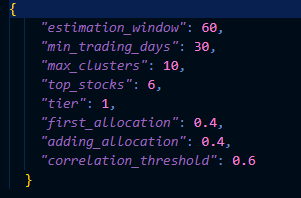
\includegraphics[width=0.8\textwidth]{insample_param.png}
    \caption{Parameters used in the in-sample backtesting.}
    \label{fig:parameters}
\end{figure}


\begin{figure}[h!]
    \centering
    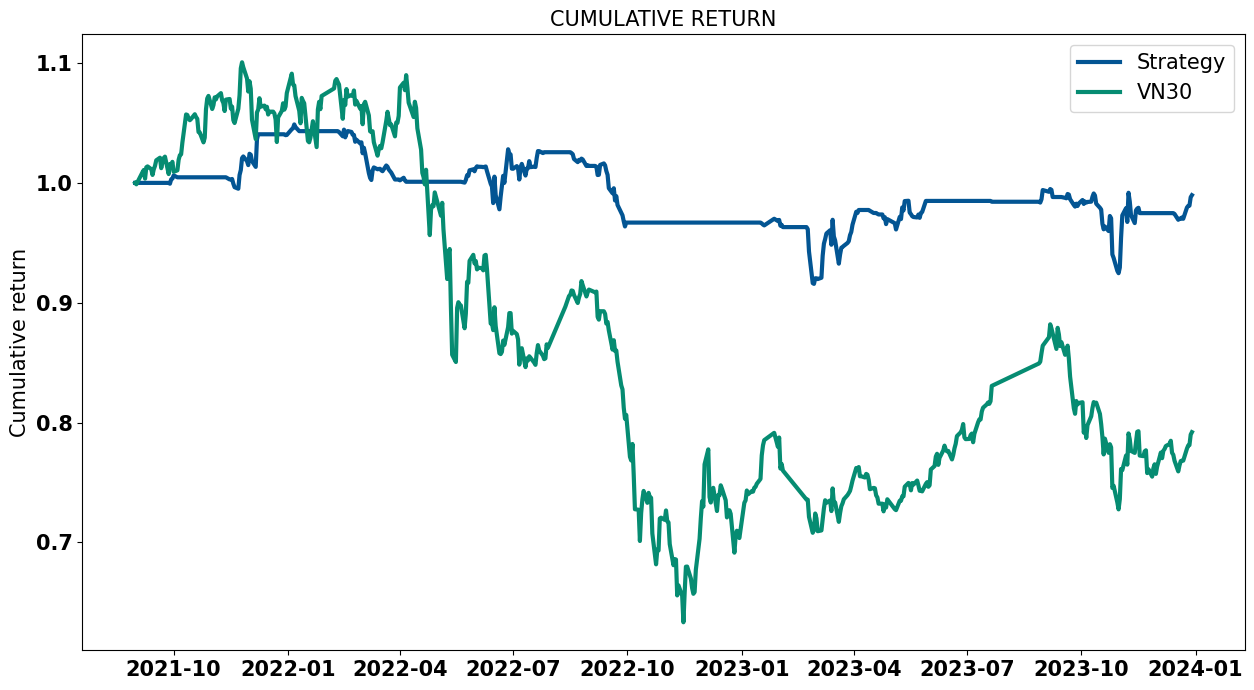
\includegraphics[width=0.8\textwidth]{insample_return.png}
    \caption{Return over time during the in-sample period.}
    \label{fig:return_over_time}
\end{figure}


\begin{figure}[h!]
    \centering
    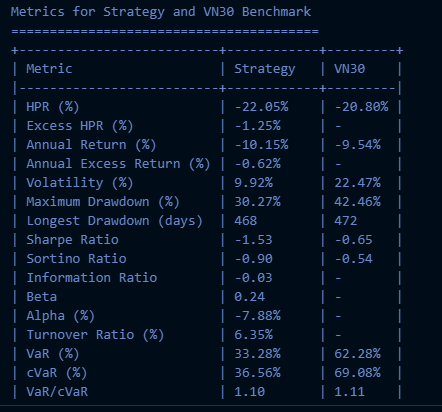
\includegraphics[width=0.8\textwidth]{insample_metrics.png}
    \caption{Key metrics evaluated for the in-sample backtesting.}
    \label{fig:key_metrics}
\end{figure}
\clearpage

\section{Optimization}
I used Optuna for the optimization part with the objective is to maximize sharpe ratio and minimize maximum drawndown.

The optimization part is somewhat flaw due to 
\begin{itemize}
    \item Limited compuational power
    \item In approriate method to avoid overfitting
    \item Limit data of VN30F1M
\end{itemize}
\begin{figure}[h!]
    \centering
    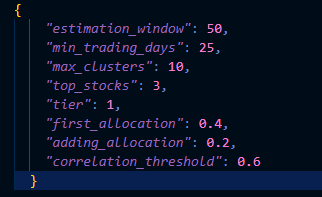
\includegraphics[width=0.8\textwidth]{optim_param.png}
    \caption{Parameters used in the optimization backtesting.}
    \label{fig:parameters}
\end{figure}


\begin{figure}[h!]
    \centering
    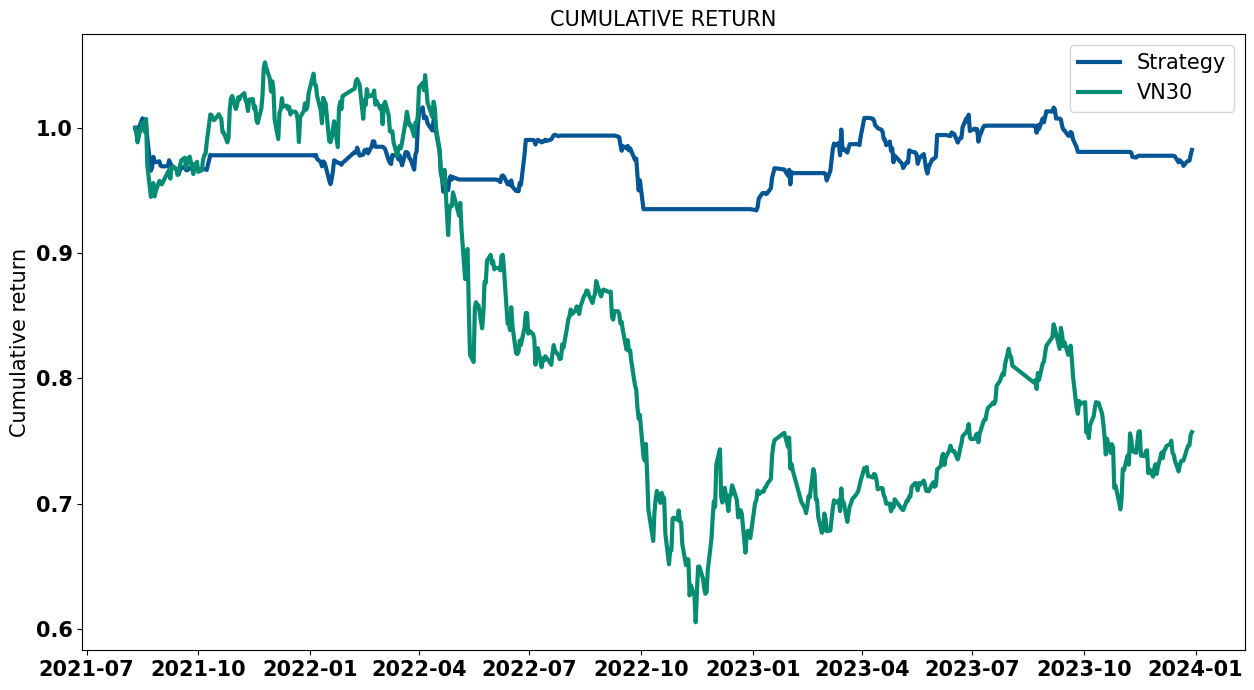
\includegraphics[width=0.8\textwidth]{op_return.png}
    \caption{Return over time during the optimization period.}
    \label{fig:return_over_time}
\end{figure}


\begin{figure}[h!]
    \centering
    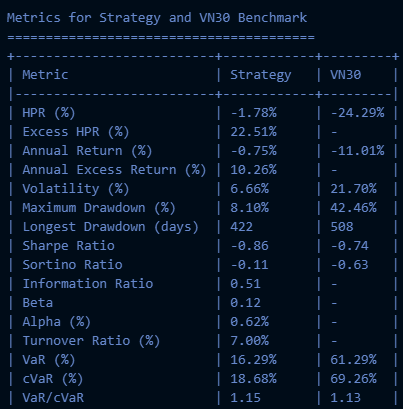
\includegraphics[width=0.8\textwidth]{optimal_metrics.png}
    \caption{Key metrics evaluated for the optimization backtesting.}
    \label{fig:key_metrics}
\end{figure}
\clearpage

\section{Out-Sample Backtesting}
The Out-Sample Backtesting poor performance is due to the overfitting in the optimization part.
\begin{itemize}
    \item Limited compuational power
    \item In approriate method to avoid overfitting
    \item Limit data of VN30F1M
\end{itemize}

\begin{figure}[h!]
    \centering
    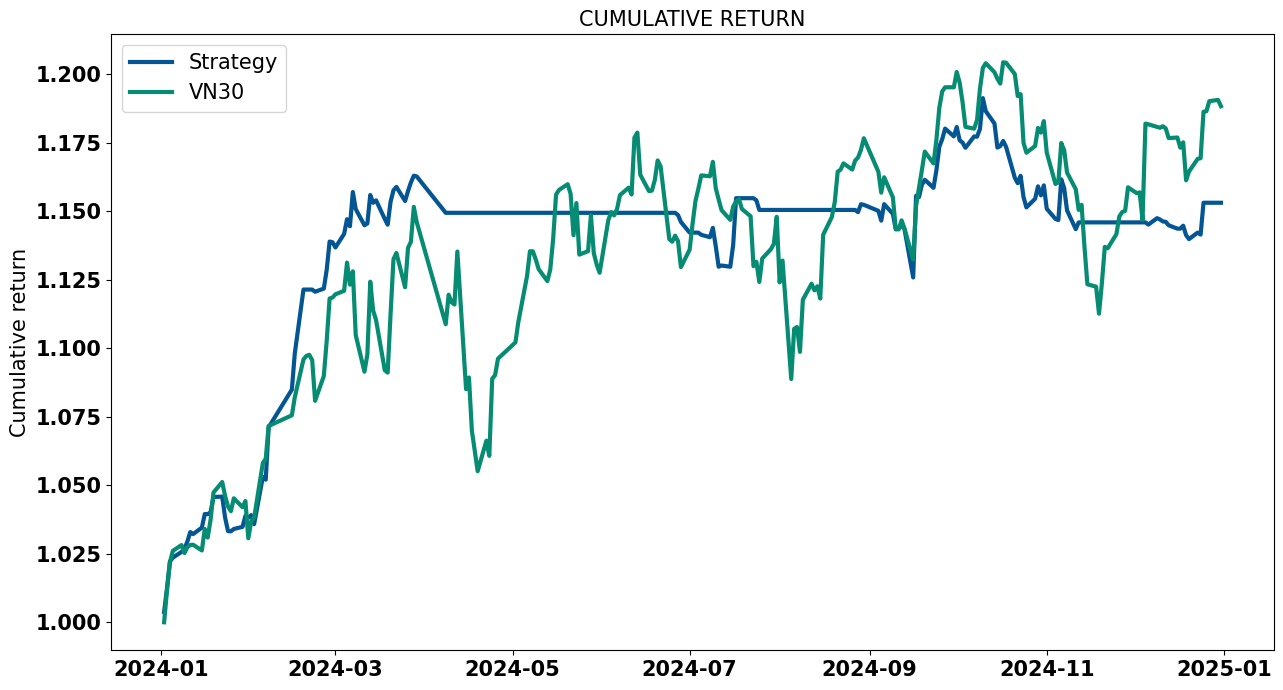
\includegraphics[width=0.8\textwidth]{outsample_return.png}
    \caption{Return over time during the out-sample period.}
    \label{fig:return_over_time}
\end{figure}


\begin{figure}[h!]
    \centering
    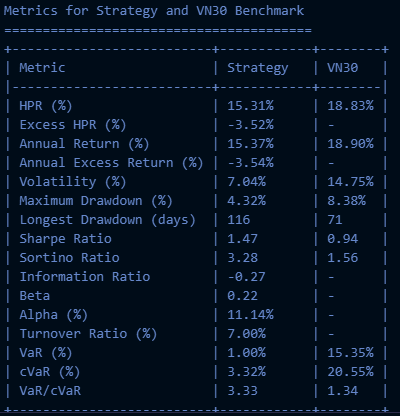
\includegraphics[width=0.8\textwidth]{outsample_metrics.png}
    \caption{Key metrics evaluated for the out-sample backtesting.}
    \label{fig:key_metrics}
\end{figure}
\clearpage

\section{Conclusion}
\subsection{Improvement}
Due to the complexity of the strategy, there are a lot of key improvements, which can lead to better result:
\begin{itemize}
    \item The forming combinations took many time and computational power, which can be further improved by more advanced methodology
    \item The result is extremely volatile with different capital-allocation-tier and their parameters. Further testing and exploring different signal generation can be made.
    \item The optimization process is not done properly due to limited computational power and in appropriate method leading to overfitting.
\end{itemize}
\subsection{Overall}
This report presents a statistical arbitrage strategy for Vietnam, overcoming short-selling restrictions by pairing stock baskets with futures. Clustering and cointegration ensure effective combination formation, while backtesting confirms potential. However, further enhancement are needed to overcome the complexity of the model.
\clearpage
\section{Appendix: Proof of Combination Formation Using Eigenvalues}
\label{app:proof}

Here, we prove how eigenvalues and eigenvectors from the Johansen test are used to form cointegrated combinations, as implemented in the code.

Consider a set of time series \(\mathbf{y}_t = (y_{0t}, y_{1t}, \ldots, y_{mt})'\), where \(y_{0t}\) is the futures price and \(y_{1t}, \ldots, y_{mt}\) are stock prices. The VECM is:

\[
\Delta \mathbf{y}_t = \Pi \mathbf{y}_{t-1} + \sum_{i=1}^{p-1} \Gamma_i \Delta \mathbf{y}_{t-i} + \mathbf{\epsilon}_t
\]

where \(\Pi = \alpha \beta'\), and \(\beta\) contains the cointegrating vectors. The Johansen test computes eigenvalues \(\hat{\lambda}_i\) and eigenvectors \(\mathbf{v}_i\) of a matrix derived from residuals of auxiliary regressions.

Suppose the largest eigenvalue \(\hat{\lambda}_1\) has eigenvector \(\mathbf{v} = (v_0, v_1, \ldots, v_m)'\). The cointegrating relationship is:

\[
\beta' \mathbf{y}_t = v_0 y_{0t} + v_1 y_{1t} + \cdots + v_m y_{mt}
\]

To express the futures as a function of the stocks with coefficient 1, normalize by \(-v_0\) (assuming \(v_0 \neq 0\)):

\[
\mathbf{\tilde{v}} = -\frac{1}{v_0} \mathbf{v} = \left(1, -\frac{v_1}{v_0}, -\frac{v_2}{v_0}, \ldots, -\frac{v_m}{v_0}\right)'
\]

Thus, the combination is:

\[
y_{0t} - \sum_{i=1}^{m} \beta_i y_{it}, \quad \text{where} \quad \beta_i = -\frac{v_i}{v_0}
\]

This linear combination is stationary if the series are cointegrated (i.e., \(\hat{\lambda}_1\) is significant). In the code, \texttt{result.evec[:, 0]} provides \(\mathbf{v}\), and betas are computed as \texttt{-evec[1:] / evec[0]}, aligning with this derivation.

\textbf{Validation}: The combination is valid if:
1. \(\beta_i \geq 0\) for all \(i\) (ensured by code checks).
2. The residuals \(y_{0t} - \sum_{i=1}^{m} \beta_i y_{it}\) are stationary (ADF test).
3. Residuals are economically reasonable (size constraint).

This proves that the eigenvectors directly yield the weights for a cointegrated portfolio, enabling the strategy to hedge the futures effectively.

\section{References}
\bibliographystyle{plainnat}
\begin{thebibliography}{9}
\bibitem{avellaneda2010}
Avellaneda, M., \& Lee, J. (2010). Statistical arbitrage in the U.S. equities market. \textit{Quantitative Finance}, 10(7), 761–782.
\bibitem{lu2018}
Lu, Y., Parulekar, A., \& Xu, J. (2018). Statistical arbitrage via cointegration and clustering. Stanford University Working Paper.
\end{thebibliography}

\end{document}

